\documentclass[problem]{mcs}

\begin{pcomments}
  \pcomment{CP_stationary_distribution}
  \pcomment{from F10.rec25}
\end{pcomments}

\pkeywords{
  stationary
  distribution
  random_walk
}

%%%%%%%%%%%%%%%%%%%%%%%%%%%%%%%%%%%%%%%%%%%%%%%%%%%%%%%%%%%%%%%%%%%%%
% Problem starts here
%%%%%%%%%%%%%%%%%%%%%%%%%%%%%%%%%%%%%%%%%%%%%%%%%%%%%%%%%%%%%%%%%%%%%

\begin{problem}
We use random walks on a digraph $G$ to model the typical movement
pattern of a Math for CS student right after the final exam.

The student comes out of the final exam located on a particular node
of the graph, corresponding to the exam room.  What happens next is
unpredictable, as the student is in a total haze.  At each step of the
walk, if the student is at node $u$ at the end of the previous step,
they pick one of the edges $\diredge{u}{v}$ uniformly at random from
the set of all edges directed out of $u$, and then walk to the node
$v$.

Let $n \eqdef \card{\vertices{G}}$ and define the vector $P^{(j)}$ to be
\[
P^{(j)}\eqdef (p_1^{(j)},\dots,p_n^{(j)})
\]
where $p_i^{(j)}$ is the probability of being at node $i$ after $j$
steps.

\bparts

\ppart\label{parta}
%\item[a.]

We will start by looking at a simple graph. If the student starts at
node 1 (the top node) in the following graph, what is
$P^{(0)},P^{(1)},P^{(2)}$?  Give a nice expression for $P^{(n)}$.
%What is the stationary distribution?

%\mfigure{!}{1.5in}{loop}
\begin{center}
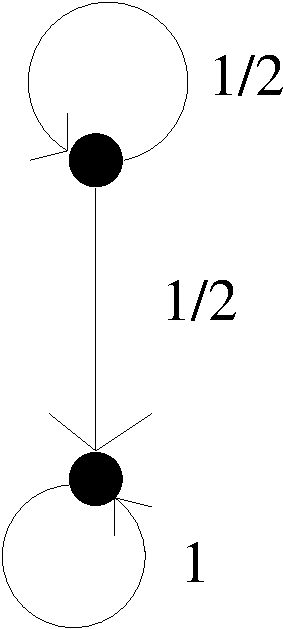
\includegraphics[height=1.5in]{loop}
\end{center}

\examspace[2in]
\begin{solution}
\[
P^{(0)} = (1,0),P^{(1)}=(1/2,1/2),P^{(2)}=(1/4,3/4),\dots, P^{(n)} = (1/2^n, 1- 1/2^n).
\]
\end{solution}

%\ppart
%Say that the graph is  {\em aperiodic} if the GCD of the
%lengths of all of the cycles in the graph is 1.    
%Is a bipartite graph aperiodic?
%
%\solution{Not unless it has only one node.}

\ppart
%\item[b.]
  Given an arbitrary graph, show how to write an expression
  for $p_i^{(j)}$ in terms of the $p_k^{(j-1)}$'s.

\examspace[2in]
\begin{solution}
We have
\[
p_i^{(j)} = \sum_{\substack{k\\ (k,i) \in E}} \frac{p_{k}^{(j-1)}}{\degr{k}}.
\]
\end{solution}

\ppart
%\item[c.]
  Does your answer to the last part look like any other
  system of equations you've seen in this course?

\examspace[1in]
\begin{solution}
It should---these are similar to the equations that we got from
PageRank!
\end{solution}

\ppart
%\item[d.]

Let the \emph{limiting distribution} vector $\pi$ be
\[
\lim_{k \rightarrow \infty} \frac{\sum_{i = 1}^{k} P^{(i)}}{k}.
\]
What is the limiting distribution of the graph from part a?
Would it change if the start distribution 
were $P^{(0)}=(1/2,1/2)$ or $P^{(0)}=(1/3,2/3)$?

\examspace[2.5in]
\begin{solution}
Say we start with the distribution $(x, 1 - x)$.  The distribution
after $i$ steps is
\[
P^{(i)} = (x/2^i, 1 - x/2^i)
\]

Plugging this into the formula for the limiting distribution, we
have

\begin{eqnarray*}
\pi & = & \lim_{k \rightarrow \infty} \frac{\sum_{i = 1}^{k} P^{(i)}}{k} \\
& = & \lim_{k \rightarrow \infty} \frac{\sum_{i = 1}^{k} (x/2^i, 1 - x/2^i)}{k} \\
& = & \lim_{k \rightarrow \infty} \paren{\frac{\sum_{i = 1}^{k} x / 2^i}{k}, \frac{\sum_{i = 1}^{k} 1 - x / 2^i}{k}} \\
& = & \lim_{k \rightarrow \infty} \paren{\frac{x - x / 2^k}{k}, \frac{k - (x - x / 2^k)}{k}} \\
& = & (0, 1)
\end{eqnarray*}
%The limiting distribution  for all of the start
%distributions is (0,1).
\end{solution}

\examspace
\ppart
%\item[e.]

Let's consider another directed graph. 
If the student starts at node 1 with probability 1/2
and node 2 with probability 1/2,
what is $P^{(0)},P^{(1)},P^{(2)}$ in the following graph?
What is the limiting distribution?

%\mfigure{!}{1.5in}{triLoop}

\begin{center}
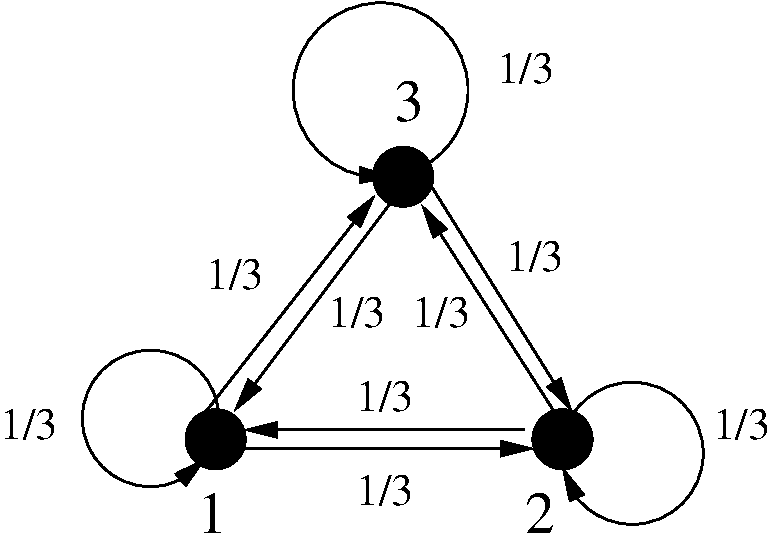
\includegraphics[width=2.5in]{triLoop}
\end{center}


\examspace[1in]\begin{solution}
$P^{(0)} = (1/2, 1/2, 0)$, $P^{(1)} = (1/3, 1/3, 1/3)$, $P^{(2)} =
  (1/3, 1/3, 1/3)$, and in general, the limiting distribution is
  $(1/3, 1/3, 1/3)$.
\end{solution}

\ppart
%\item[f.]
  Now we are ready for the real problem.  In order to make it
  home, the poor Math for student is faced with $n$ doors along a long
  hall way.  Unbeknownst to him, the door that goes outside to
  paradise (that is, freedom from the class and more importantly,
  vacation!) is at the {\em very end}.  At each step along the way, he
  passes by a door which he opens up and goes through with probability
  1/2.  Every time he does this, he gets teleported back to the exam
  room.  Let's figure out how long it will take the poor guy to escape
  from the class.  What is $P^{(0)},P^{(1)},P^{(2)}$?  What is the
  limiting distribution?

%\mfigure{!}{1.5in}{lineMark}

\begin{center}
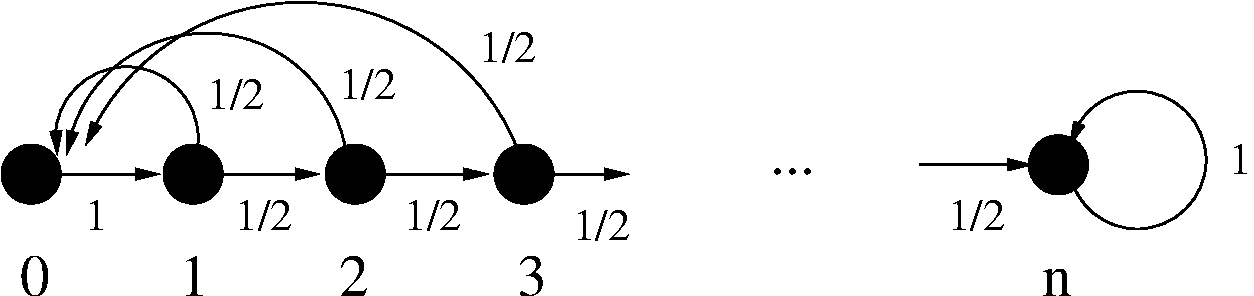
\includegraphics[width=4.5in]{lineMark}
\end{center}

\examspace[1.5in]
\begin{solution}
$P^{(0)}$ just has $p_0^{(0)} = 1$ and all other probabilities $0$,
  since the student is at the exam room and has just
  started. $P^{(1)}$ just has $p_1^{(1)} = 1$ since the student made
  the only move possible, and all other probabilities $0$. $P^{(2)}$
  has $p_0^{(2)} = 1/2$, since the student opens the first door with
  probability $1/2$, and $p_2^{(2)} = 1/2$, since the student passes
  the first door with probability $1/2$.

Eventually, we reach node $n$, at which point we stay there
forever. Thus, the limiting distribution has $p_i = 0$ for $i = 0, 1,
\ldots, n-1$, and $p_n = 1$.
\end{solution}

\ppart
%\item[g.]
  Show that the expected number $T(n)$ of teleportations
  you make back to the exam room before you escape to the outside
  world is $2^{n-1}-1$.

\begin{solution}

The probability that you manage to reach the last door to the outside
without getting teleported back to the 6.042 exam room is
$\frac{1}{2^{n-1}}$.  Thus, by the mean time to failure formula,
$T(n)$, the expected number of times you get teleported back to the
6.042 exam room is $2^{n-1}-1$ (on the last try you don't get
teleported back, but rather, you succeed.)

\end{solution}

\iffalse
\ppart
%\item[h.]

The poor 6.042 student has a friend that
also took the exam, and thinks he did very well on it.
The friend brags that he can use Markov's inequality
to upper bound the probability that the 6.042 student gets
teleported back to the 6.042 exam room more than
$6T(n)$ times before he finally escapes.  What bound
can he get?

\begin{solution}

Using Markov's inequality, the probability is at most $1/6$.

\end{solution}

\ppart
%\item[i.]

At first the poor 6.042 student wants to push his friend
into the first teleportation black hole that he can find.
But, then the poor 6.042 student thinks hard and realizes
that he can get a much better and much easier upper bound
on the probability that he (the poor 6.042 student) gets
teleported back to the 6.042 exam room more than
$6T(n)$ times before he finally escapes.  What bound
can he get?

\begin{solution}

The probability that the 6.042 student
does not escape by the time he gets teleported 
$s$ teleportations is
$(1-2^{-n})^{s}$. So, the probability that he
does not escape by time $6T(n)$ is at most
$(1-2^{-n})^{6T(n)} =(1-2^{-n})^{62^n} = e^{-6}$. 

\end{solution}

\fi

\eparts

\end{problem}

%%%%%%%%%%%%%%%%%%%%%%%%%%%%%%%%%%%%%%%%%%%%%%%%%%%%%%%%%%%%%%%%%%%%%
% Problem ends here
%%%%%%%%%%%%%%%%%%%%%%%%%%%%%%%%%%%%%%%%%%%%%%%%%%%%%%%%%%%%%%%%%%%%%

\endinput
 
